% Working draft based on the approved Chinese manuscript and author revisions.
% 2026-11-08: Method (3), Listening Data Construction (4), Experiments (5).
% Task is nested in Method; evaluation remains nested in Experiments.
% Compile with XeLaTeX. Chinese author notes are intentionally visible.
\documentclass[10pt,twocolumn,letterpaper]{article}
\usepackage[review]{cvpr}
\usepackage{xeCJK}
\IfFontExistsTF{Noto Serif CJK SC}
  {\setCJKmainfont{Noto Serif CJK SC}}
  {\setCJKmainfont[BoldFont=FandolSong-Bold]{FandolSong-Regular}}
\IfFontExistsTF{Noto Sans CJK SC}
  {\setCJKsansfont{Noto Sans CJK SC}}
  {\setCJKsansfont[BoldFont=FandolHei-Bold]{FandolHei-Regular}}
\usepackage{tabularx,array,makecell}
\usepackage{placeins}
\definecolor{cvprblue}{rgb}{0.21,0.49,0.74}
\definecolor{authorblue}{RGB}{40,81,125}
\newif\ifauthornotes
\authornotestrue
% Chinese planning notes: keep visible in this authoring draft.
\newcommand{\cnnote}[2]{\ifauthornotes\par\smallskip{\small\upshape\color{authorblue}\noindent\textbf{【#1】}#2\par}\smallskip\fi}
\newcommand{\pending}{\textcolor{authorblue}{\textsf{TBD}}}
\newcommand{\NA}{\textsf{N/A}}
\newcommand{\on}{\ensuremath{\checkmark}}
\newcommand{\off}{\ensuremath{-}}
\newcolumntype{Y}{>{\raggedright\arraybackslash}X}
\newcommand{\figdraft}[1]{\textbf{#1 (draft).}}
\graphicspath{{figures/}}
% Do not hide layout defects behind the template's 30pt tolerance.
\hfuzz=0pt
\vfuzz=0pt

\usepackage[pagebackref,breaklinks,colorlinks,allcolors=cvprblue]{hyperref}
\def\confName{CVPR}
\def\confYear{2027}
\title{Audiovisual Backchannel Generation During Listening}
\author{Anonymous Authors}
\begin{document}
\maketitle
\begin{abstract}
\cnnote{摘要待写}{按中文稿约定，待主张、正式实验和结果稳定后撰写摘要。当前标题只用于识别任务，尚非最终标题。本版为英文正文与中文作者备注并存的工作稿；表中的TBD表示尚未填写，不代表零分；图中示意素材不作为实验结果。}
\end{abstract}

% 2026-11-08: revised from the author's version, not from the initial draft.
% Exact author version and change rationale: review/intro_revision_20261108/.
% Citation keys are stable placeholders; replace matching entries in references.bib.
\section{Introduction}
\label{sec:intro}

% Paragraph role P01: 任务价值与成功标准——倾听行为是否合适，而不仅是媒体是否逼真。
Natural conversation requires both speaking and listening. While one
participant holds the conversational floor, the listener conveys attention
and engagement through facial expressions, head movements, and brief vocal
acknowledgments~\cite{learningtolisten,omnipersona}. These backchannels
support the ongoing utterance without taking over the conversation. Visual
reactions may occur with or without vocal feedback, and quiet listening is
also appropriate. Digital humans therefore need to produce appropriate
listening behavior as well as fluent spoken responses: realistic faces and
voices alone do not establish whether feedback fits the conversational
context.

\begin{figure*}[t]
\centering
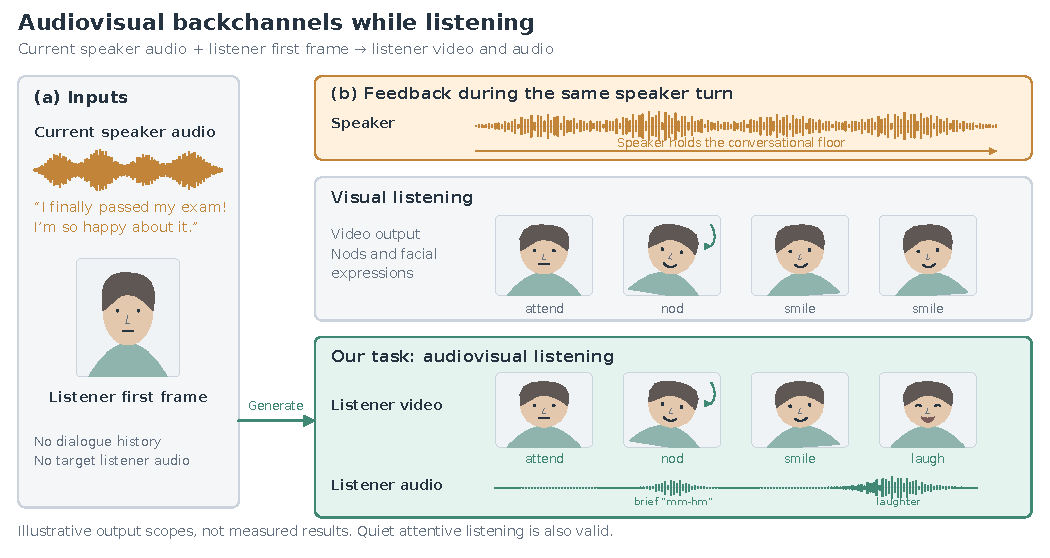
\includegraphics[width=\textwidth]{F1_task.pdf}
\caption{\figdraft{F1: Audiovisual backchannels during listening} Given current speaker audio and the listener's first frame, the task is to generate listener video and audio while the speaker holds the floor. Quiet listening is also valid. The rows illustrate visual and audiovisual output scopes, not measured comparisons between methods. Portraits, utterances, and waveforms are schematic.}
\label{fig:task}
\end{figure*}

% Paragraph role P02: 已有能力递进——给定目标语音、视觉倾听、双音轨交互、自主视听回应。
Speech-driven talking-head methods such as
OmniHuman-1.5~\cite{omnihuman15} synthesize visual behavior from the target
person's supplied speech. Listening-generation methods, including
ViCo~\cite{vico}, Learning to Listen~\cite{learningtolisten}, and
GLARE~\cite{glare}, instead generate visual reactions to another speaker
without synthesizing the listener's audio. 
% GLARE also introduces reaction-oriented supervision and evaluation.
Interactive methods such as INFP~\cite{infp} and DyStream~\cite{dystream}
model speaking and listening from both participants' audio tracks, with
the target person's vocal behavior supplied as an input. OmniResponse~\cite{omniresponse}
and OmniPersona~\cite{omnipersona} further generate audiovisual
conversational responses, including listener feedback. Building on these
advances, we focus on listening feedback as the primary target of learning
and evaluation, and investigate how listening-specific conditioning,
supervision, and data can support its visual and vocal expression.
% 引用边界：不推断OmniResponse／OmniPersona只做整段对话评价；两者已有倾听反馈研究。

% Paragraph role P03: 任务设定及应用理由——无需用户视频，允许无历史的初次／独立交流。
We study audiovisual backchannel generation from the current speaker audio
and a reference image of the listener (\cref{fig:task}). This setting
supports interaction with a visible digital avatar without requiring the
user to enable a camera, and accommodates initial or standalone exchanges
with no prior dialogue history. 
% The image specifies the avatar's visual identity, while the current utterance provides the conversational input.
The listener's audio is generated rather than supplied: the model must
produce visual reactions, brief vocal feedback, and quiet listening while
the speaker retains the floor.

% Paragraph role P04: 两个建模挑战——从对方语音构建生成条件，以及显式监督短暂反馈行为。
Learning this behavior presents two related challenges. First, the input
speech belongs to the other participant: it provides semantic and acoustic
cues, but does not prescribe the listener's articulation or reaction.
These cues must be mapped to conditions suitable for generating the
listener's audio and video. Second, feedback can be brief, subtle, and
interspersed with quiet listening. A media-generation objective supervises
the audiovisual output as a whole, but does not explicitly specify which
feedback categories should occur. This motivates event supervision that
makes feedback behavior a direct target of learning.
% 这是本文的设计依据，不是对所有既有模型已验证的失败结论。

% Paragraph role P05: 方法回应挑战——直接声学条件＋目标特征适配，对应第一个挑战；Event对应第二个。
Our framework addresses these challenges through direct speaker-audio
conditioning and supervision of both conditioning representations and
feedback events. Speaker-audio cross-attention supplies acoustic
information to the generator, while target audiovisual feature supervision
trains the conditioning mapping to retain information relevant to the
listener's response. Clip-level event supervision complements the
media-generation objective by encouraging the corresponding feedback
categories to occur. This auxiliary objective supervises category presence
over the clip without imposing exact event timestamps.
% Feature监督适配条件映射，不更新冻结Qwen；整段Event不表示其他AV训练目标也放弃时间对应。
% 效果待证据：上述句子说明机制与目标，不预填组件收益或联合优于级联的结论。

% Paragraph role P06: 数据回应学习要求——角色更新、配对媒体和有序视听反应描述。
To support listening-focused learning, we construct paired
audiovisual data from Seamless conversations~\cite{seamless},
updating speaker--listener roles as turns change while retaining
brief vocal backchannels as listening feedback. We use extracted
visual and vocal cues to guide Qwen3-Omni~\cite{qwen3omni} in
producing ordered reaction descriptions, linking speaker audio
with listener audiovisual media and annotations of their feedback.

% Paragraph role P07: 评价回应任务标准——类别一致性、语境／参与感、生成音画自身协调。
We formulate a listening-focused evaluation design that considers
audiovisual quality, feedback-category agreement, contextual
appropriateness and engagement, and audiovisual coordination. A speaker
utterance can admit multiple reasonable reactions~\cite{learningtolisten,reactface},
so agreement with one recorded response cannot fully determine feedback
quality. Clip-level category agreement measures whether the reference
feedback categories are expressed without requiring temporal overlap with
reference events. Contextual evaluation considers whether a response fits
the utterance and preserves the listening role, including reasonable
alternatives to the reference; audiovisual coordination concerns the
relation between generated sounds and movements. Together, these
dimensions separate media quality from the listening behavior it conveys.
% GLARE也承认一对多；这里的区别是类别一致性不要求时间重叠，不是首次提出一对多。
% 后续计划仍为中文：类别／检测器、人工量表及正式结果未定，故使用evaluation design。

% Paragraph role P08: 贡献收束——保留作者的模型、数据、评价顺序。
Our contributions are as follows:
\begin{itemize}
    \item We introduce an audiovisual backchannel generation framework
    conditioned on current speaker audio and a listener reference image.
    It combines direct acoustic conditioning, target audiovisual feature
    supervision, and clip-level event supervision for listening feedback.

    \item \textcolor{red}{(如果写数据贡献，需要一些体现贡献的数字：xxh，xxpairs，xxtypes…)}We construct listening-focused audiovisual data through
    role-aware clip pairing and cue-assisted feedback annotation,
    associating speaker audio with listener audiovisual media and ordered
    descriptions of visual and vocal behavior.

    \item We formulate a listening-focused evaluation design that
    complements audiovisual quality with feedback-category agreement,
    contextual appropriateness and engagement, and audiovisual
    coordination, accommodating reasonable variation in listener responses.
\end{itemize}




% 11-07
% \section{Introduction}
% \label{sec:intro}
% % Paragraph role P01: 开场：任务及目标
% Speakers and listeners both contribute to natural conversation. Listeners use nods, facial expressions, and brief vocal acknowledgments to convey attention and engagement. Digital humans therefore need to produce natural audiovisual feedback while listening. We study audiovisual backchannel generation from the current speaker audio and a reference image of the listener, with the aim of making conversation more natural and engaging (\cref{fig:task}).

% \begin{figure*}[t]
% \centering
% 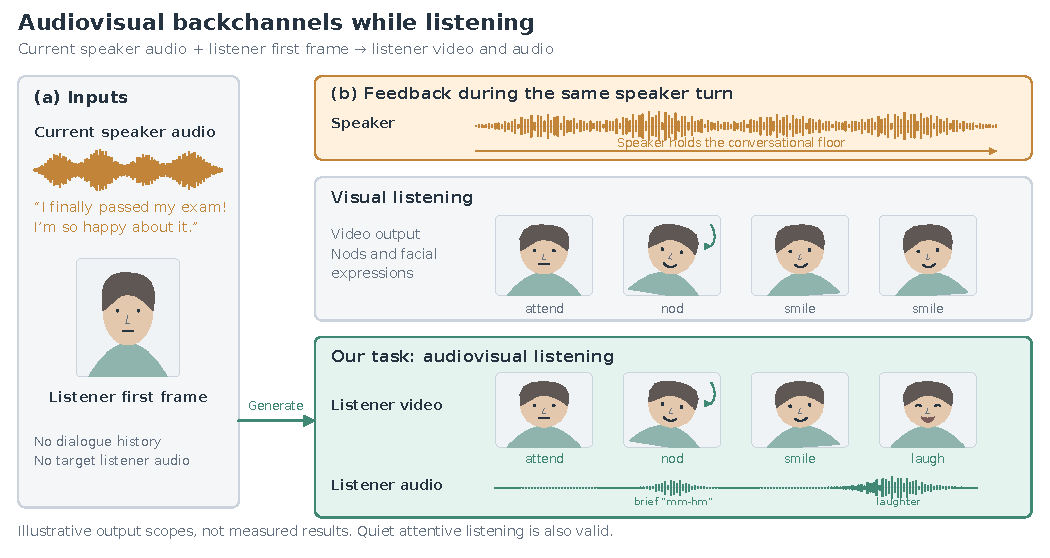
\includegraphics[width=\textwidth]{F1_task.pdf}
% \caption{\figdraft{F1: Audiovisual backchannels during listening} Given current speaker audio and the listener's first frame, the task is to generate listener video and audio while the speaker holds the floor. Quiet listening is also valid. The rows illustrate visual and audiovisual output scopes, not measured comparisons between methods. Portraits, utterances, and waveforms are schematic.}
% \label{fig:task}
% \end{figure*}

% % Paragraph role P02: 已有能力与本文范围
% Speech-driven talking-head methods, such as OmniHuman-1.5~\cite{omnihuman15}, generate facial motion from the target person's given speech, emphasizing lip synchronization and natural motion. Listening-generation methods instead model responses to a speaker. ViCo~\cite{vico}, Learning to Listen~\cite{learningtolisten}, and GLARE~\cite{glare} generate visual listening behavior without generating the listener's own audio. More recent work, including OmniResponse~\cite{omniresponse} and OmniPersona~\cite{omnipersona}, also studies vocal and silent responses. We focus on feedback produced while the speaker holds the conversational floor, using only the current speaker audio and the listener's reference image, without dialogue history or a supplied listener audio track.

% % Paragraph role P03: 技术困难与设计目标
% This task requires converting semantic and acoustic information in the current speech into listener sounds and visual behavior. General multimodal representations provide a basis for understanding, but their mapping to audiovisual generation conditions still needs to be adapted to listening. Moreover, media reconstruction objectives do not directly specify whether feedback categories, such as nods or acknowledgments, should occur. We therefore address the use of current speech information, the adaptation of conditioning representations, and explicit supervision of feedback behavior.

% % Paragraph role P04: 数据需求
% The task also requires paired speaker inputs, listener video, and the listener's own audio, with clear listening roles and feedback annotations. Existing resources support these requirements to different extents. Some do not provide an independent listener audio track ready for generation training. Others contain both participants' audiovisual information but still require listening-oriented sample organization and backchannel annotation. Converting raw conversations into suitable training samples thus requires task-specific data preparation.
% \cnnote{待补引用}{上述资源差异沿用中文稿的限定表述。定稿时须为各类局限补充对应资源证据；不将Seamless或ResponseNet写成完全没有音轨或行为标注。}

% % Paragraph role P05: 评价需求
% Evaluation must also address listening behavior. Standard video-quality metrics describe visual fidelity and realism, but a visually convincing output may still lack meaningful feedback or respond inappropriately to the current utterance. Evaluation should therefore consider audiovisual quality, feedback behavior, naturalness, and conversational engagement.

% % Paragraph role P06: 数据方案
% We address these requirements through data construction, a generation framework, and an evaluation design. Starting from Seamless conversations~\cite{seamless}, we use pauses, ASR punctuation, and transcript-based utterance-boundary cues to organize paired speaker--listener clips. To address reaction omissions observed when describing audiovisual clips directly, we extract visual and vocal cues and provide their categories and temporal intervals to Qwen3-Omni~\cite{qwen3omni}. The resulting natural-language descriptions organize reactions in their observed order, providing paired media and descriptions for learning audiovisual listening responses.

% % Paragraph role P07: 方法方案
% Our generator uses speaker-audio cross-attention to supply direct acoustic information, target audiovisual feature supervision to adapt the conditioning representations, and clip-level event supervision to encourage the corresponding backchannel categories. These components address input information, condition adaptation, and feedback expression, respectively.
% \cnnote{证据待补}{这里陈述设计目的；三个组件的实际效果由最终同条件消融支持，不预写显著提升或最优结论。}

% % Paragraph role P08: 评价方案
% Our evaluation design considers clip-level event-category agreement, contextual appropriateness and engagement, and audiovisual event coordination. Category agreement allows feedback timing to vary, contextual evaluation allows different reasonable responses, and coordination concerns the relation between generated sounds and movements.
% \cnnote{协议待补}{测试集组织、事件检测与核验、人工评价工具及细则尚待确定；不表示完整benchmark已执行或发布。}

% % Paragraph role P09: 贡献入口
% Our contributions are as follows:
% \begin{itemize}
% \item We construct paired data for audiovisual backchannel generation during listening from Seamless conversations. Role-aware clip organization, media processing, and cue-assisted annotation link speaker audio, listener audiovisual media, and ordered reaction descriptions.
% \item We introduce a generation framework conditioned on current speaker audio and the listener's first frame. Direct audio conditioning supplies acoustic information, target feature supervision adapts the conditioning representations, and clip-level event supervision explicitly encourages feedback categories.
% \item We organize feedback evaluation around clip-level category agreement, contextual appropriateness and engagement, and audiovisual coordination, complementing media-quality evaluation while allowing reasonable variation in reaction timing.
% \end{itemize}
% \cnnote{贡献边界}{第三条保留为已确认的评价设计，不新增“首个”“首次”或“已发布benchmark”的主张。本文仅说明采用联合生成，不主张其已被证明优于音频—视频级联。}

\section{Related Work}
\label{sec:related}
\subsection{Audiovisual Conversation and Response Generation}
% Paragraph role P01: 视觉倾听沿革
Listening-generation methods synthesize facial expressions and head movements from a speaker's communication signals. ViCo~\cite{vico} introduces responsive listening-head generation and paired data, using speaker audiovisual signals and a preset attitude to generate listener motion. Learning to Listen~\cite{learningtolisten} models listener motion as a nondeterministic distribution, allowing multiple responses to the same input. Subsequent work explores diffusion-based diverse generation, emotion control, and text-based customization through MFR-Net~\cite{mfrnet}, ELP~\cite{elp}, and CustomListener~\cite{customlistener}, respectively. DiffListener~\cite{difflistener} and DiTaiListener~\cite{ditailistener} further develop expressive listening-video generation.

% Paragraph role P02: 行为适当性与事件表示
Beyond visual quality, ReactFace~\cite{reactface} studies online generation of multiple appropriate facial reactions, considering appropriateness, diversity, and synchrony. GLARE~\cite{glare} represents reactions as events with categories and temporal intervals, combining prosodic conditioning, temporal reaction supervision, and event evaluation. These visual listening methods provide a basis for behavior modeling, but do not generate the listener's own audio. Our task includes brief acknowledgments and laughter together with the corresponding video, while retaining silent listening as a valid output.

% Paragraph role P03: 已知音轨的交互视频
Interactive-avatar methods also differ in whether the target audio is supplied or generated. INFP~\cite{infp} and DyStream~\cite{dystream} use both participants' audio tracks to generate avatar videos that include speaking and listening. ARIG~\cite{arig} additionally models interaction using both participants' audiovisual signals and dialogue states. These methods incorporate role changes and listening into generation, but receive the target person's audio as a condition. Our model must generate both listener audio and video from the other person's current speech and a listener reference frame.

% Paragraph role P04: 自主AV回应与本文边界
OmniResponse~\cite{omniresponse} is closer to this setting: it uses speaker facial information, transcripts, and dialogue history to generate aligned text and facial responses, with TempoVoice synthesizing audio for vocal responses. OmniPersona~\cite{omnipersona} encodes multimodal conversation history into linguistic and non-linguistic conditions and jointly generates audio and video, including listening backchannels and identity consistency across turns. Audiovisual listening responses therefore already have a research basis. Our focus is feedback during the other person's turn from a short current audio segment and a listener first frame, without dialogue history, speaker video, a target listener audio track, or a reference voice. We address this setting through direct audio conditioning, target feature supervision, and clip-level event supervision, rather than introducing a multi-turn memory task.

\subsection{MLLM-Based Cascaded Generation}
\cnnote{中文待补：作者已确认的新结构}{本小节尚无写定正文，先保留中文。后续结合OmniPersona对理解与生成框架的介绍，核实“MLLM理解／规划→文本或隐表征→生成器”的代表工作、接口与条件，再写文献介绍。不能把所有条件接口统称为同一种级联；Qwen→OVI系统对照也不等于先生成音频再驱动视频。这里不新增“联合生成优于级联”的主张，暂不补造文献或技术关系。}

\subsection{Conversation Data and Feedback Evaluation}
% Paragraph role P05: 数据资源及本文组织
Existing datasets cover different aspects of dyadic interaction. ViCo~\cite{vico} provides listening-generation samples. RealTalk~\cite{realtalk} contains natural dyadic conversations with transcripts and active-speaker annotations, while Seamless Interaction~\cite{seamless} provides large-scale face-to-face interaction data. SpeakerVid-5M~\cite{speakervid} organizes dialogue, listening, and multi-turn branches; its listening branch pairs speaker audio with silent listener video. ResponseNet, introduced with OmniResponse~\cite{omniresponse}, provides synchronized videos of both participants, multichannel audio, transcripts, and facial behavior annotations. GLARE~\cite{glare} adds visual reaction categories and temporal intervals. These resources already provide paired media and several types of behavior annotation. Their support for our task depends on clip organization, role definitions, and coverage of vocal feedback. We further organize Seamless into speaker-held-turn clips with aligned listener audiovisual media, and use timestamped visual and vocal cues to obtain ordered reaction descriptions.

% Paragraph role P06: 既有评价与本文协议
Feedback evaluation has also moved beyond visual quality. REACT2023~\cite{react2023} and ReactFace~\cite{reactface} consider multiple appropriate reactions. GLARE evaluates category matches with temporal overlap. OmniResponse and SpeakerVid-5M assess multimodal response quality and audiovisual synchronization, while OmniPersona also evaluates the appropriateness of listening expressions. Building on these dimensions, our evaluation design separates clip-level event-category agreement, contextual appropriateness and engagement, and coordination within generated audiovisual feedback. Clip-level agreement does not require alignment with one reference's event times, but cannot by itself establish contextual appropriateness. The three dimensions address short, intermittent feedback that may have multiple reasonable realizations.
\cnnote{引用与审阅}{本节为中文相关工作草稿的英文整理，仍待作者审阅。GLARE和OmniPersona沿用提供稿件，不推断作者或录用信息；正式BibTeX按引用清单补齐。}

% Method verified against the current AV + Whisper + Feature + LTX clip-Event code.
% Source map, equations, and remaining author decisions: review/方法重写与实现核对_20261108.md.
\section{Method}
\label{sec:method}

\begin{figure*}[t]
\centering
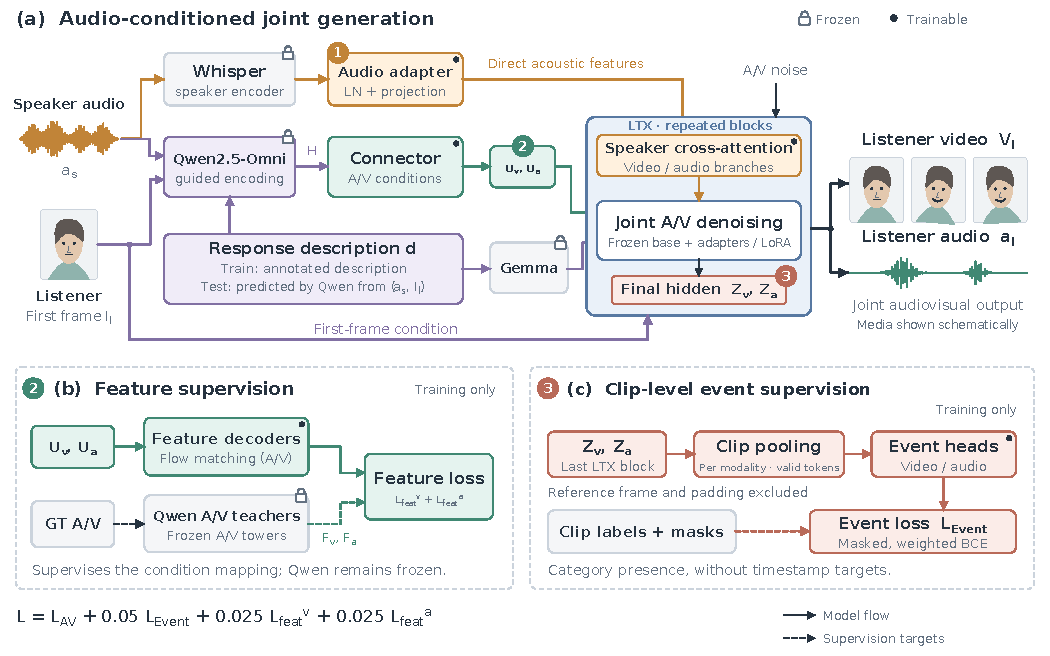
\includegraphics[width=\textwidth]{F3_method.pdf}
\caption{\figdraft{F3: Generation framework and training supervision} A connector maps guided Qwen representations to video and audio conditions, which are appended to Gemma text conditions. An independent Whisper path supplies speaker-audio features to both LTX streams. Feature supervision trains the condition mapping with frozen target-media features; clip-level Event supervision reads the final LTX block. Training uses annotated descriptions, whereas inference predicts and re-encodes descriptions from the permitted inputs. Both auxiliary objectives are used only during training. Portraits and waveforms are schematic.}
\label{fig:method}
\end{figure*}

\subsection{Task Definition and Overview}
\label{sec:conditioning}
% Included inside Method 3.1 by 05_method.tex; this file adds no numbered heading.
\label{sec:task}
\paragraph{Task definition.}
% Paragraph role P01: 任务——当前语音与首帧到同时间段的倾听视听反馈。
Given the current speaker audio $a_s$ and the listener's first frame $I_l$,
we generate listener video $V_l$ and audio $a_l$ over the corresponding
interval. We focus on feedback while the speaker holds the conversational
floor, including facial reactions, head movements, and brief vocal
acknowledgments. Quiet listening is also valid. The input does not uniquely
determine the listener's reaction or its timing, and an observed response
is one possible realization. At inference, the model receives no dialogue
history, speaker video, target listener audio, or reference reaction labels.
\cnnote{统计待补}{应用面向一两句当前话语；训练与测试的实际片段长度及句数分布仍需报告，不能把应用设定直接写成已统计确认的数据分布。}

% Paragraph role P02: 监督接口——先说明方法使用哪些数据，构建细节放第4章。
Training uses paired listener audiovisual media, an ordered reaction
description $d^*$, and clip-level behavior labels with validity masks.
These descriptions and labels are derived from the target media during
data construction (\cref{sec:data}); they are supervision, not additional
inputs required from the user.


\paragraph{Generation conditions.}
% Paragraph role P01: 总览——理解条件、直接声学条件与联合生成器的分工。
Our framework combines a description-conditioned representation of the
intended response with direct acoustic information from the speaker
(\cref{fig:method}). A frozen Qwen2.5-Omni model~\cite{qwen25omni} encodes
the speaker audio, listener image, and a reaction description $d$ into
multilayer hidden states $H$. A trainable connector $C_\theta$ produces
separate video and audio conditions, while Gemma~\cite{gemma_pending}
encodes the same description. For modality $m\in\{v,a\}$, we write
\begin{equation}
 (U_v,U_a)=C_\theta(H),\qquad c_m=[G_m(d);U_m],
\label{eq:conditions}
\end{equation}
where $G_m(d)$ is the processed Gemma context for that stream and brackets
denote token concatenation. The joint LTX generator~\cite{ltx_pending}
uses $c_v$, $c_a$, the reference frame, and the speaker-audio features
introduced below to generate both listener modalities.

% Paragraph role P02: Connector——层感知记忆与坐标查询将Qwen表征映射到两路条件。
The connector normalizes and projects each selected Qwen layer into a
shared memory, adding learned layer embeddings before concatenation.
Video and audio queries are initialized from feature-grid coordinates
and modality embeddings. Each fusion block applies cross-attention to
the Qwen memory, self-attention across the combined query sequence, and
a feed-forward network. Separate output projections produce $U_v$ and
$U_a$ in the dimensions required by the two LTX context streams. This
provides a trainable interface between frozen understanding and generation
models. The final projection topology follows Bernini~\cite{bernini_pending};
the coordinate-query fusion defines how information is gathered from the
selected Qwen layers.

% Paragraph role P03: 描述来源——训练用标注，推理预测并重新编码，描述是内部条件。
During training, $d=d^*$ is the annotated description of the target
response. It is appended as assistant guidance after Qwen's multimodal
input prefix, and the resulting sequence supplies $H$. During inference,
Qwen first predicts $\hat d$ from $a_s$, $I_l$, and the task instruction;
we then re-encode this description to obtain $H$ and $G_m(\hat d)$.
The description is thus an internal condition. Direct acoustic
conditioning supplements this representation, while Feature and Event
supervision respectively target the condition mapping and generated
feedback behavior.

\subsection{Direct Speaker-Audio Conditioning}
\label{sec:direct-audio}
% Paragraph role P04: Whisper动机与设计——保留直接声学信息，补充描述与高层条件。
A reaction description summarizes intended behavior, but does not
explicitly preserve every local acoustic cue in the speaker's utterance.
We therefore provide a separate path from speaker audio to the generator.
A frozen Whisper-large-v3 encoder~\cite{whisper} extracts a temporal
feature sequence; a trainable LayerNorm and linear adapter map it to
speaker context $S$. Independent cross-attention branches inject $S$
into the video and audio streams of every LTX block:
\begin{equation}
 h_{b,m}\leftarrow h_{b,m}
 +\operatorname{CA}_{b,m}(h_{b,m},S),\quad m\in\{v,a\},
\label{eq:speaker-attention}
\end{equation}
where $b$ indexes a block. Generation features provide queries, and
speaker features provide keys and values. These branches supplement
the existing attention to $c_m$ in \cref{eq:conditions}.

% Paragraph role P05: 时间与初始化——共同时间坐标、保留静音、无额外Whisper损失。
Speaker keys and generation queries use temporal rotary positions
defined on a common time origin in seconds. Padding is masked, and
leading and internal speaker silence are retained. The additional output
projections are initialized to zero, preserving the original path at
initialization. The adapter and attention branches learn through the
generation and Event objectives; there is no separate Whisper loss.
The model can attend to the supplied audio segment as a whole and does
not impose streaming causality.

\subsection{Target Audiovisual Feature Supervision}
\label{sec:feature}
% Paragraph role P06: Feature动机——让实际送入生成器的条件携带目标媒体信息。
The connector must transform general multimodal representations into
conditions useful for listener generation. To supervise this mapping,
we extract target features $F_v$ and $F_a$ from real listener video and
processed audio using frozen Qwen visual and audio encoders. The queries
that produce $U_m$ are organized to correspond to these teacher-feature
positions. An auxiliary decoder $D_{\phi_m}$ for each modality learns
to recover target features conditioned on $U_m$, following the
AdaLN-modulated feature-decoder design of Bernini~\cite{bernini_pending}.

% Paragraph role P07: Feature公式——独立噪声下的特征流匹配，保留有效位置与安静音频。
For each valid feature position, we sample Gaussian noise $\epsilon$
and a noise level $\sigma\sim\mathcal U(0,1)$, forming
$x_{\sigma,m}=(1-\sigma)F_m+\sigma\epsilon$. The decoder predicts
the flow velocity toward noise, with objective
\begin{equation}
 \mathcal L_{\mathrm{Feature}}^m =
 \mathbb E_{\sigma,\epsilon}\!\left[
 \big\|D_{\phi_m}(x_{\sigma,m},\sigma,U_m)
       -(\epsilon-F_m)\big\|_{\Omega_m}^{2}\right].
\label{eq:feature}
\end{equation}
Here the squared norm averages over channels and positions in
$\Omega_m$, where both the teacher feature and condition are valid;
the training loss is also averaged over samples. Silence is a valid
audio target and is not excluded solely because no vocalization occurs.

% Paragraph role P08: Feature梯度——监督Connector，冻结Qwen，推理无需教师或解码器。
Because the decoders consume the same $U_m$ used by LTX, their gradients
encourage the connector to retain information relevant to the target
listener media. This is a conditional feature-reconstruction objective,
not a direct regression between Qwen hidden states and teacher features.
The connector and auxiliary decoders are trainable; the Qwen backbone
and teacher encoders remain frozen. Neither target features nor auxiliary
decoding is required at inference.

\subsection{Clip-Level Event Supervision}
\label{sec:event}
% Paragraph role P09: Event动机与读出——从生成表征而非条件U监督反馈类别存在。
The continuous audiovisual objective does not explicitly specify which
feedback categories should occur. We therefore attach visual and audio
event heads to the generation representations of LTX. In each training
forward pass, we read hidden states $Z_v$ and $Z_a$ from the final
Transformer block, before output normalization and projection. Video
states are averaged spatially within each valid time position and then
temporally; audio states are averaged over their valid temporal positions.
Pooling excludes reference-frame tokens, padding, and positions outside
the actual generation support. Separate LayerNorm--MLP heads map the
pooled representations to clip-level category logits.

% Paragraph role P10: Event标签与公式——区分正例、弱负例和未知，按有效样本归一化。
The targets are derived from reaction descriptions with the evidence
checks described in \cref{sec:annotation}. For sample $i$ and class $c$,
$y_{ic}\in\{0,1\}$ denotes category presence, $M_{ic}$ indicates a valid
target, and $w_{ic}$ controls its weight. Accepted positives have weight
1; unmentioned categories receive weak-negative weight 0.1 only when
the description passes the completeness checks. Uncertain or conflicting
entries are masked. We use class-weighted binary cross-entropy:
\begin{equation}
 \mathcal L_{\mathrm{Event}}=
 \frac{1}{|\mathcal C_{\mathrm{eff}}|}
 \sum_{c\in\mathcal C_{\mathrm{eff}}}
 \frac{\sum_i M_{ic}w_{ic}\,
       \mathrm{BCE}_{\alpha_c}(s_{ic},y_{ic})}
      {\sum_i M_{ic}},
\label{eq:event}
\end{equation}
where $s_{ic}$ is a logit, $\alpha_c$ is a positive-class weight derived
from training statistics, and $\mathcal C_{\mathrm{eff}}$ contains enabled
classes with valid targets in the training batch. Normalization uses the
number of valid samples rather than their weight sum, preserving the
reduced influence of weak negatives.

% Paragraph role P11: Event作用边界——整段存在性适配可变时序，但不保证所有生成行为正确。
This objective supervises whether a category occurs within the clip,
without imposing event start or end times. It accommodates variation in
feedback timing while the audiovisual objective continues to supervise
the paired media. Event heads read hidden states at the sampled
flow noise level, so training requires no additional full video sampling
or decoding. Their gradients pass through the trainable LTX branches to
the connector. The heads are not executed at inference; their predictions
are not used to score generated videos. The training behavior vocabulary
and the evaluation categories are defined separately.

\subsection{Training and Inference}
\label{sec:training}
\paragraph{Joint objective.}
% Paragraph role P12: AV目标——双路潜空间流匹配，固定参考首帧并屏蔽无效支持。
The native audiovisual objective trains LTX to jointly predict video and
audio flow velocities. Let $x_0^m$ be a target latent encoded by the frozen
modality VAE. At a sampled noise level $\tau$, we form
$x_\tau^m=(1-\tau)x_0^m+\tau\epsilon_m$ at generated positions.
The reference-frame latent stays clean and fixed. Writing the joint
generator's output for stream $m$ as $v_\Theta^m$, the loss is
\begin{equation}
 \mathcal L_{\mathrm{AV}}=
 \mathbb E\!\left[
 \sum_m
 \big\|v_\Theta^m(x_\tau^v,x_\tau^a,\tau;\mathcal K)
       -(\epsilon_m-x_0^m)\big\|_{\Lambda_m}^{2}\right],
\label{eq:av}
\end{equation}
where $\mathcal K$ collects the reference-frame, Qwen/Gemma, and Whisper
conditions. $\Lambda_m$ is the valid generation mask, excluding fixed
reference positions and padding; the norm is a mean over valid positions
and channels, and the expectation includes training samples and noise.

% Paragraph role P13: 总目标——Whisper是条件路径，Feature与Event是辅助监督。
The complete model uses
\begin{equation}
\begin{split}
 \mathcal L ={}& \mathcal L_{\mathrm{AV}}
       +0.05\mathcal L_{\mathrm{Event}}\\
       &+0.025\mathcal L_{\mathrm{Feature}}^v
        +0.025\mathcal L_{\mathrm{Feature}}^a.
\end{split}
\label{eq:total}
\end{equation}
We train the connector, Whisper adapter and attention branches, auxiliary
feature decoders, event heads, and LoRA adapters in LTX's native video and
audio text cross-attention. The Qwen, Gemma, Whisper, and VAE encoders,
target-feature teachers, and pretrained LTX backbone weights remain
frozen. Feature supervision acts on the condition mapping; Event
supervision reaches that mapping through the generation network.

\paragraph{Inference.}
% Paragraph role P14: 推理——预测描述、构建条件、联合采样，保持训练外目标不可见。
Given $a_s$ and $I_l$, Qwen predicts $\hat d$ and re-encodes it to construct
the guided hidden states; Gemma encodes the same description. The
connector produces $U_v$ and $U_a$, while Whisper supplies direct speaker
features. LTX jointly samples video and audio latents from noise, keeping
the reference-frame latent fixed, and decodes the listener response.
Both classifier-free guidance branches retain the Qwen and Whisper
conditions; the negative branch uses empty Gemma text. No target listener
media, annotated descriptions, teacher features, or event labels are
accessed. Model versions and sampling settings are specified in
\cref{sec:setup}.

\section{Listening Data Construction}
\label{sec:data}
% Section role: explain how paired media, descriptions, and labels are constructed.

\begin{figure*}[t]
\centering
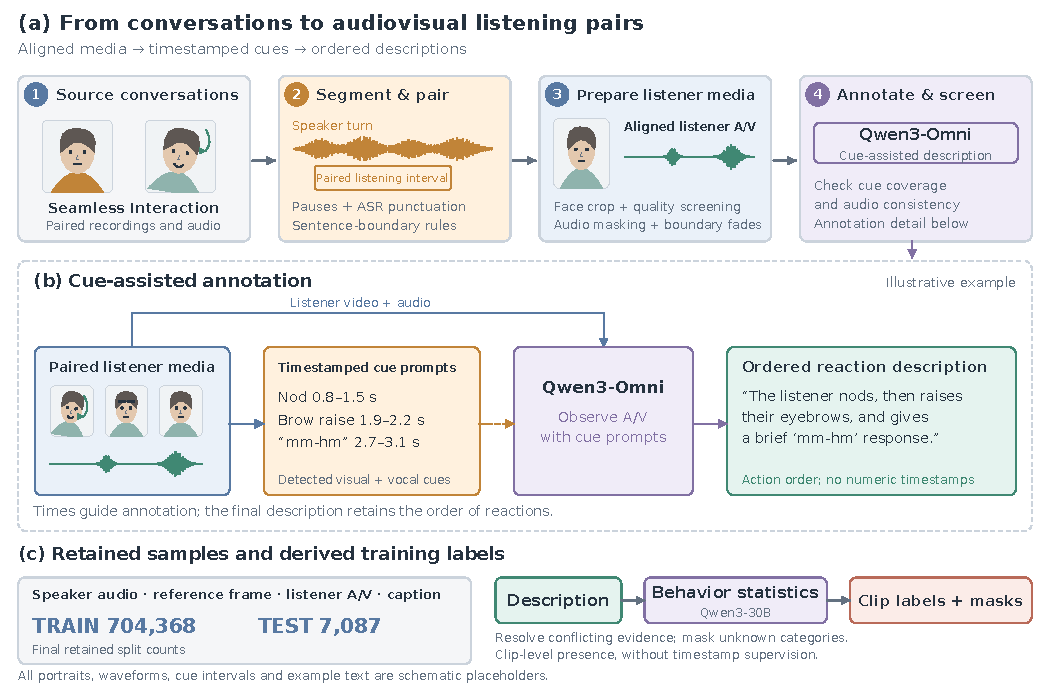
\includegraphics[width=\textwidth]{F2_data.pdf}
\caption{\figdraft{F2: Data construction and cue-assisted annotation} Seamless conversations are segmented and paired before listener media processing. Listener audiovisual media and timestamped reaction cues guide Qwen3-Omni to produce an ordered description without numerical timestamps. Each sample links the input conditions, listener targets, and description. Text-based behavior extraction and conflict masking produce clip-level training labels. Example media, cue intervals, and descriptions are schematic; the reported resource counts differ from the AV training selection.}
\label{fig:data}
\end{figure*}
\subsection{Role-Aware Pair Construction}
\label{sec:pairing}
\paragraph{Source and conversational roles.}
% Paragraph role P01: 数据来源及目标
We construct paired listening data from Seamless conversations~\cite{seamless}. The source recordings contain alternating speaking turns, whereas our task requires identifying the current speaker, the corresponding listener, and their feedback during the same interval. We associate speaker audio, a listener reference frame, and aligned listener audiovisual targets, and add natural-language descriptions of visual and vocal reactions. \Cref{fig:data} summarizes the process.

% Paragraph role P02: 切分与角色规则
We use transcripts, word timings, speech activity, and acoustic pauses to determine local roles and candidate boundaries. When the listener takes over the conversational floor, we switch the roles and continue forming pairs, allowing both participants' speaking turns to contribute samples. Brief listener feedback may overlap with speaker speech and does not automatically indicate a turn change. Segmentation favors complete sentence endings and avoids including a fragment of the next sentence. Longer content is split at valid boundaries. The fixed rules limit clips to 2--11.95 seconds and treat an inter-word pause longer than 5 seconds as a long-pause boundary. Candidate formation precedes audio-quality filtering and, where needed, local recovery; cases whose recovered subsegments cannot be confirmed as complete are retained for review.
\cnnote{范围与细则}{此处的语义线索指转写与句末完整性规则，不表示调用大模型进行语义切分，也不表示每个片段覆盖一个完整长话轮。角色判定阈值、来源构成和原始资源许可待补。原始会话采集不归为本文贡献。}

\paragraph{Aligned listener media.}
% Paragraph role P03: 媒体处理
We screen and crop listener video and correct orientation in affected source clips. Reaction detection and audiovisual annotation use the same person, crop, and temporal interval. For audio, we extract the corresponding interval from the listener's independent long audio track. The union of official word, utterance, and voice-activity intervals defines the retained regions. We extend these regions by 100\,ms on each side and apply 10\,ms fades to reduce boundary discontinuities and interference from other sounds. Audio outside the retained regions is zeroed rather than removed, preserving duration and audiovisual alignment. Source media, crop, and processing metadata are retained for subsequent inspection.
\cnnote{质量证据待补}{100毫秒和10毫秒是音频保留区间的处理参数，不是所有视频切口的统一余量。处理输入为512×512不表示原始素材具有同等有效分辨率；净化、裁剪和角色配对的质量需独立抽检。}

\subsection{Cue-Assisted Reaction Annotation}
\label{sec:annotation}
\paragraph{Ordered reaction descriptions.}
% Paragraph role P04: 线索辅助描述
Direct audiovisual descriptions were observed to omit some movements and brief vocal reactions. We therefore extract candidates such as nods, head shakes, brow lowering, and brow raising from listener video. Within officially supported vocal intervals, ASR, official transcripts, and audio events provide vocal cues. Cue categories, start and end times, and available vocal content are supplied to Qwen3-Omni~\cite{qwen3omni}, together with the listener video sampled at 8\,fps using the final crop and the processed audio. The prompt directs attention to transient reactions and requests an ordered account of visual and vocal behavior. The output is an English natural-language description that preserves reaction order without numerical timestamps. The pipeline checks cue coverage and consistency with silence, retries suspected omissions, and retains unresolved review flags.

% Paragraph role P05: 表情线索与时间证据限制
These cues describe observable behavior: brow movements do not directly establish an internal emotional state. Their intervals are annotation prompts, not manually verified event boundaries.
\cnnote{待补证据}{需通过独立核验比较有／无辅助线索的描述，分别检查遗漏、无依据添加及顺序错误。流程设计不能直接支持“完整性和顺序准确性已提升”的效果结论。}

\paragraph{Clip-level training labels.}
% Paragraph role P06: 描述派生整段标签
A separate, fixed behavior-extraction procedure uses Qwen3-30B-A3B-Instruct-2507~\cite{qwen3} to extract visual and audio behavior names with supporting text from the descriptions. Accepted items provide positive evidence for clip-level category presence. Uncertain, contradictory, or insufficiently supported items remain unknown. A category is treated as a low-weight negative only when the description passes a completeness check and genuinely does not mention it. Conflicts involving mentioned baseline states, supplementary reaction cues, and weak negatives are masked. If vocal activity is supported but its subtype is uncertain, all audio categories are not labeled absent. This step adds no temporal supervision, and the automatic labels are not treated as human ground truth.

\subsection{Dataset Statistics}
\label{sec:data-statistics}
% Paragraph role P07: 样本与规模
Each sample links the current speaker audio, the listener's first frame, aligned listener video and audio, and a reaction description, together with source and temporal metadata. The retained resource contains 704,368 training samples and 7,087 test samples. The AV generation model uses a separately selected training set, specified in \cref{sec:setup}; these counts do not denote the same training manifest. Data and annotation quality checks are organized in \cref{sec:validation}.
\begin{table*}[t]
\centering\small
\begin{tabularx}{\textwidth}{@{}lYY@{}}
\toprule
Resource & Available support & Relation to listening feedback \\
\midrule
ViCo~\cite{vico} & Paired listening samples and attitudes & Visual listening generation \\
RealTalk~\cite{realtalk} & Dyadic video, transcripts, active-speaker labels & Conversation source \\
Seamless~\cite{seamless} & Dyadic audiovisual media and aligned annotations & Source of our paired clips \\
SpeakerVid-5M~\cite{speakervid} & Dialogue, listening, multi-turn branches & Listening branch: speaker audio and silent listener video \\
ResponseNet~\cite{omniresponse} & Both videos, multichannel audio, transcripts, facial annotations & Audiovisual response resource \\
GLARE~\cite{glare} & Paired clips and timed visual reaction labels & Visual event supervision and evaluation \\
Our organization & Paired speaker audio, listener media, ordered descriptions & Listening-phase audiovisual feedback \\
\bottomrule
\end{tabularx}
\medskip
\begin{tabular}{@{}lrr@{}}
\toprule
Resource / usage & Clips & Duration (hours) \\
\midrule
Retained resource: train & 704,368 & \pending \\
Retained resource: test & 7,087 & \pending \\
AV generation training selection & 284,218 & $\approx 500$ \\
\bottomrule
\end{tabular}
\caption{Data resources and retained samples. Resource counts and the AV training selection refer to different manifests.}
\label{tab:data}
\end{table*}

\cnnote{资源关系待核对}{704,368／7,087沿用中文D5的全量筛选口径；生成模型使用284,218段AV选集，不能自行假定它是704,368条中的严格子集。正式测试及校准清单、人物隔离、行为分布和人工质量抽检待补。}

\section{Experiments}
\label{sec:experiments}
\cnnote{本节状态}{实验结构与五组消融已确认，正式结果尚未汇齐。下面把已确定的比较问题写成英文，将执行计划、版本核对和待做内容保留中文。表T1--T4为筹备编号；正式排版编号由LaTeX生成。所有结果表仅展示结构，不预填成绩。}

% Paragraph role P01: 实验证据链——整体能力、组件作用和资源／评价可信度。
The experimental design addresses three questions: how the model performs on audiovisual backchannels and shared visual-listening capabilities, what each component contributes, and how reliably the data and evaluation capture listening behavior.

\subsection{Experimental Setup}
\label{sec:setup}
\paragraph{Training data and test settings.}
% Paragraph role P02: 实际AV训练集与测试范围
Generation training uses a separately selected set of 284,218 clips totaling approximately 500 hours. This selection includes source training data and part of the source development split; the latter is not an independent validation set. These are the AV training counts, distinct from the retained resource statistics in \cref{sec:data-statistics}.
\cnnote{测试清单待冻结}{Seamless固定200作为同源AV评价候选，ResponseNet分层随机200作为跨来源候选，ViCo test43作为视觉补充。三者不自动构成新benchmark。需确定模型选择／阈值校准／最终测试清单，核查同源对话、时间重叠及人物身份；隔离结论按实际证据报告。D5的最终资源数量不等于本节正式benchmark规模。}
\cnnote{抽样与泄漏}{早期“48条非零音频＋按模型表现选出的152条”只作探索，不作无偏主测试。多次用于选模型的诊断集需披露用途。测试保留有声／安静的自然分布，单独有声子集按预定义规则组织。}

\paragraph{Implementation details.}
% Paragraph role P03: 已确认模型版本与训练实现
Generation training uses frozen Qwen2.5-Omni-3B without planning SFT, with hidden states from layers 8, 18, 28, and 35. The generator is LTX-2.3-22B, and the speaker encoder is Whisper-large-v3. Qwen3-Omni is used separately for data annotation. The connector has four fusion blocks of width 1,024 with 16 attention heads; its video and audio outputs have dimensions 4,096 and 2,048. The auxiliary feature decoders each use 16 AdaLN residual blocks of width 1,024 to predict 2,048-dimensional teacher features. LTX text-attention LoRA uses rank and scaling parameter 8. Precomputed conditions, target features, and labels refer to the same selected media.

% Paragraph role P04: Event实现口径——训练词表、启用门槛与评测词表分开。
The Event heads have 16 visual and 3 audio output slots. Eighteen classes meet the validity criteria and the minimum support of 5,000 positive examples; the mouth-closing slot is retained but excluded from the loss. This training vocabulary contains general visual behaviors and is separate from the communicative categories used in evaluation.
\cnnote{引用与配置待补}{上述结构及维度已按当前配置和实际复用源码核对。Gemma的正式模型版本、LTX与Bernini的正式书目信息仍需补齐；源码定位见配套方法核对文档。生成训练中的Qwen未做规划SFT。}
\cnnote{采样设置待冻结}{中文稿当前共享推理函数采用30步采样，视频／音频CFG为3／7。它们是可在实验中统一调整的参数，不是方法贡献。最终检查点、规划器及采样协议须共同确定后填写。}
\cnnote{版本待冻结}{当前生成训练使用base Qwen hidden；最新LTX6000／6500＋SFT2752评测由SFT模型预测描述并重新提取H，属于“训练base H、推理SFT H”的配置。若最终主表采用该版本，须说明规划SFT及条件切换，并在所有对照中统一；本轮不把SFT自动并入AV＋Whisper＋Feature＋Event的四项设计。最终检查点、规划器和预算仍需冻结，不同batch／步数的终点不能直接当作等预算。}

\paragraph{Baselines and common protocol.}
\cnnote{完整AV候选}{优先安排本文A0／A1及Qwen2.5-Omni→OVI系统对照。后者需适配允许安静和短反馈，固定模型与prompt，不能使用真实caption、事件或listener音轨。OmniResponse、OmniPersona、SpeakerVid-5M目前尚未获得可执行原生成器，先保留文献比较，不复制原表分数到本文短pair表。}
\cnnote{视觉与额外输入对照}{GLARE需重训并披露Tref及previous motion来源；DyStream将self audio置零，Avatar Forcing将self audio和user视觉置零。L2L、DualTalk等保留额外动作／音轨条件时单列表，纯动作结果只在同表示空间比较；未核验renderer前不纳入视频表。RLHG、DIM、ReactFace、ListenFormer、LFI为资源允许时的扩展，不全部列为必做。}
\cnnote{共同协议}{统一片段范围、参考帧、分辨率／帧率、音量处理、采样预算和失败处理，不用GT挑best-of-N。OVI1.1单次上限10秒而本任务可达11.95秒，需选择全部方法的共同窗口或公开分段／拼接协议，不能只截短基线。}
\cnnote{原论文数值}{原协议文献表与本地实测分开。BFM/L1、EMOCA／DECA距离和不同含义的FD不混排；各论文RealTalk划分不视为统一测试。官方权重迁移、本文重训、第三方重实现及引用分别标注；协议不一致不计算相对提升。FID/FVD使用统一特征汇总，不平均分片分数。}

% Metrics are defined once here; results below refer back to this protocol.
% Included by 07_experiments.tex as Section 5.2; do not also load from main.tex.
\subsection{Evaluation Protocol}
\label{sec:evaluation}

\begin{figure*}[t]
\centering
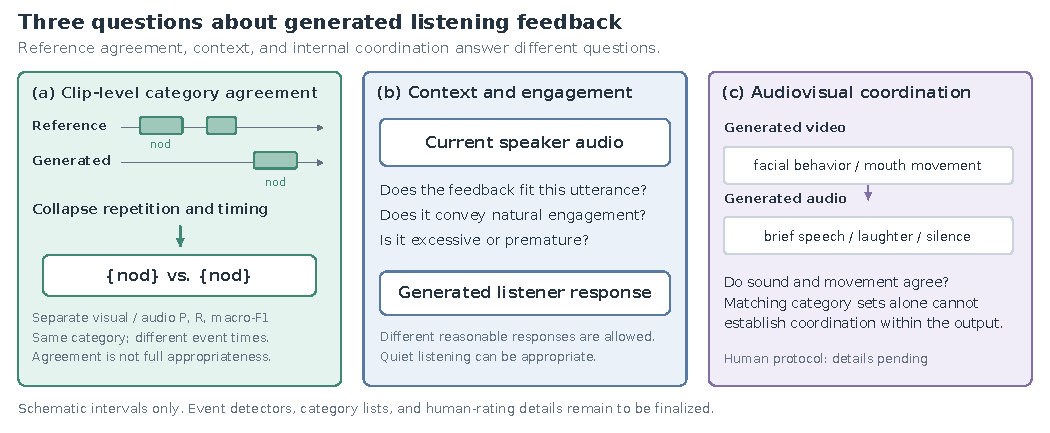
\includegraphics[width=\textwidth]{F4_evaluation.pdf}
\caption{\figdraft{F4: Evaluation design} Clip-level category agreement removes the requirement to reproduce reference event times. Separate judgments address appropriateness under the current utterance and coordination within generated audio and video. Matching categories alone cannot establish either property. Event intervals are schematic; detectors and human-rating details remain to be specified.}
\label{fig:evaluation}
\end{figure*}
% Paragraph role P01: 总体评价设计
We extend an evaluation framework based on OmniResponse~\cite{omniresponse} with measures for listening feedback. The design considers media quality, visual behavior, and vocal activity, alongside three interaction dimensions: clip-level event-category agreement, contextual appropriateness and engagement, and audiovisual event coordination.
\cnnote{实现范围}{这是本地扩展的评测框架，不表示完全复现OmniResponse作者原表。三组评价方向已确认；整段语义事件与人工评价的完整执行细则仍待落实。}

\paragraph{Clip-level event-category agreement.}
% Paragraph role P02: 一对多时序动机
An utterance often constrains the affective or attitudinal direction of a response. Smiling or shared laughter may be natural after happy news, while a head shake can express disagreement. Even when responses have similar intent, listeners can nod, smile, or vocalize at different pauses, with different durations and repetition counts. Requiring overlap with a single reference's event intervals may therefore penalize an appropriate category expressed at a different time.

% Paragraph role P03: 类别一致性及局限
We collapse repeated instances of a category within a clip into a presence label and compute precision, recall, and macro-F1 separately for visual and audio categories. The comparison does not require temporal overlap between generated and reference events. It measures category agreement with the observed response, rather than event-localization accuracy. Affect does not uniquely determine behavior: happy news need not always elicit laughter. Category agreement therefore cannot recognize every reasonable response by itself. Allowing variation relative to reference timing also does not make premature, prolonged, or internally uncoordinated feedback acceptable. \Cref{fig:evaluation} illustrates these distinct questions.
\cnnote{待定技术关系}{最终类别表、外部检测器、阈值、未知标签处理与核验方式未定。P/R的汇总口径尚未写明，不自行假定为micro或macro；Macro-F1沿用已确认表述。训练Event头的类别也不直接作为最终评测类别表。}

\paragraph{Video quality and visual behavior.}
% Paragraph role P04: 视频指标定义
Paired video evaluation includes PSNR, SSIM, LPIPS, FID, FVD, Emo-Acc, Emo-Div, and $\Delta$Resp. PSNR and SSIM measure pixel and structural similarity; LPIPS measures perceptual distance; FID and FVD compare image and video feature distributions. Following the definitions used by AnyTalker~\cite{anytalker}, Emo-Acc measures agreement between predicted seven-class expression labels on jointly valid face frames. Emo-Div counts distinct predicted expression classes per video; generated and reference values are reported separately, without assuming that larger values are better. $\Delta$Resp measures the difference in average eye-and-brow movement magnitude during listening, weighted by phase duration.

% Paragraph role P05: 视频指标解读边界
These measures provide complementary observations, not complete judgments of interaction. Emo-Acc is frame-level reference agreement, not contextual emotional correctness. $\Delta$Resp does not directly measure nod counts, eye contact, or semantic appropriateness. Framewise similarity describes differences from one reference and does not exclude other valid responses.
\cnnote{指标引用待补}{LPIPS、FID、FVD、表情工具及其他实际使用指标的原始论文引用需按实现核对后补齐。本版不编造书目信息，也不依据相同指标名混用不同实现。}

% Paragraph role P06: GLARE补充协议
The framework also integrates GLARE's R-F1, R-tIoU, R-ATD, and R-FID~\cite{glare} for supplementary visual-reaction and temporal-alignment diagnostics. GLARE's R-F1 requires category and interval matching, so it is distinct from our clip-level category F1.

\paragraph{Vocal activity, audio quality, and synchronization.}
% Paragraph role P07: 声音活动定义及局限
For brief, intermittent listener sounds, the implementation distinguishes energy-based acoustic activity from speech detected by a voice-activity detector. It supports activity-duration error, the fraction of reference-vocal clips with an entirely missed response, extra vocal time during reference silence, and false vocalization on entirely silent clips. Acoustic activity may include laughter or humming, but can also include noise; it is not itself a semantic backchannel event. Strict and tolerant interval-matching precision, recall, F1, and boundary errors provide additional timing diagnostics, separate from clip-level semantic category agreement.

% Paragraph role P08: 适用音质与同步
For continuous speech windows that satisfy their input requirements, UTMOSv2 assesses audio quality and SyncNet's LSE-D and LSE-C assess synchronization between mouth motion and generated sound. Very short acknowledgments, non-speech vocalizations, and silent clips may not support these measures.
\cnnote{评测执行要求}{对不可测项报告N/A和有效覆盖率，不通过重复或拼接短回应获得分数。这类样本仍保留声音活动与行为评价。UTMOSv2和SyncNet的正式引用、适用窗口及最终报告项按实际实现补齐。}

\paragraph{Contextual appropriateness and audiovisual coordination.}
% Paragraph role P09: 语境与声画协调
The design considers whether feedback fits the current speaker audio, is natural without being excessive, and conveys listening engagement. It also considers whether generated sounds and movements form a coordinated response, such as laughter accompanying a smiling face. Different reasonable responses and natural quiet listening are allowed. The human-assessment design is described in \cref{sec:qualitative}.
\cnnote{人工评价待完成}{这两组初步采用人工评价，具体评分形式未定。后续分别设置语境适当性、参与感／自然度及视听协调维度，不能将问卷工具就绪写成已收集人工结果。}
\cnnote{保留的中文执行要求}{评价针对最终生成的音视频进行，不以训练辅助头的分类结果替代生成效果。各项分数同时报告有效样本或窗口覆盖率；未知标签、检测失败与真正无事件分开处理，不将不可测项填为零或满分。}
\cnnote{已有执行与待补}{视频八项及声音活动已有双200结果；最新6000步结果中UTMOSv2因参考语音过短而无有效窗口。SyncNet与GLARE指标已接入工具，但该轮未运行。整段语义事件指标与人工评价待实施。}


\subsection{Quantitative Comparisons}
\label{sec:quantitative}
\paragraph{Audiovisual backchannel generation.}
% Paragraph role P05: 完整视听任务的比较范围
The full-task comparison concerns listener audio, visual reactions, and their coordination (\cref{tab:av}). It uses current speaker audio and a listener first frame as inputs and does not treat supplied listener audio as generated audio.
\cnnote{比较所能支持的结论}{已知listener音轨的动画对照只评价驱动画面；独立OVI的共享预测文本对照评价生成器，Qwen→OVI端到端对照评价系统，两者均不替代三组件消融。不同训练来源的迁移结果不能解释为共同训练下的架构因果优势。}
\cnnote{定量结果待写}{完成同协议比较后，先写主表支持的最重要发现，再说明对应的媒体质量、反馈类别和声音诊断证据；如指标有取舍，明确写出。当前不预设本文优于基线。}
\begin{table*}[t]
\centering\small
\caption{T2a: Audiovisual comparison layout. All scores are unfilled. Inputs are current speaker audio and the listener's first frame; no target listener audio is supplied. The Qwen--OVI row is a candidate system comparison pending adaptation. $n$ denotes the applicable sample or window count; exact metric coverage is to be reported separately.}
\label{tab:av}
\setlength{\tabcolsep}{5pt}
\begin{tabularx}{\textwidth}{@{}Yrrrrrrr@{}}
\toprule
& \multicolumn{3}{c}{Visual quality} & \multicolumn{3}{c}{Audio diagnostics / quality} & \\
\cmidrule(lr){2-4}\cmidrule(lr){5-7}
Method & FID$\downarrow$ & FVD$\downarrow$ & LPIPS$\downarrow$ & \makecell{Miss$\downarrow$\\(\%)} & \makecell{False$\downarrow$\\(\%)} & UTMOS$\uparrow$ & $n$ \\
\midrule
A0: Base & \pending & \pending & \pending & \pending & \pending & \pending & \pending \\
A1: Full & \pending & \pending & \pending & \pending & \pending & \pending & \pending \\
Qwen$\rightarrow$OVI & \pending & \pending & \pending & \pending & \pending & \pending & \pending \\
\bottomrule
\end{tabularx}
\medskip
\begin{tabularx}{\textwidth}{@{}Yrrrrrrrr@{}}
\toprule
& \multicolumn{4}{c}{Visual events} & \multicolumn{4}{c}{Audio events} \\
\cmidrule(lr){2-5}\cmidrule(lr){6-9}
Method & P$\uparrow$ & R$\uparrow$ & mF1$\uparrow$ & $n_v$ & P$\uparrow$ & R$\uparrow$ & mF1$\uparrow$ & $n_a$ \\
\midrule
A0: Base & \pending & \pending & \pending & \pending & \pending & \pending & \pending & \pending \\
A1: Full & \pending & \pending & \pending & \pending & \pending & \pending & \pending & \pending \\
Qwen$\rightarrow$OVI & \pending & \pending & \pending & \pending & \pending & \pending & \pending & \pending \\
\bottomrule
\end{tabularx}
\cnnote{表头与条件待冻结}{Miss对应参考有声片段的整段漏回应比例，False对应完全静音片段上的误发声比例；这两项是参考一致性诊断，不直接判断合理性。P/R汇总口径未定，mF1指Macro-F1。训练来源、检查点、输入适配、短声指标有效覆盖和逐类支持数待补；无有效音质窗口时填N/A。不同测试集分别填同结构面板，不混合排名。}
\end{table*}


\paragraph{Shared visual-listening capabilities.}
% Paragraph role P06: 视觉对照与额外输入边界
The visual comparison concerns capabilities shared with video-only listening methods (\cref{tab:visual}). Methods that require additional inputs or produce only motion are considered separately; their results do not establish performance on the full audiovisual task.
\begin{table*}[t]
\centering\small
\caption{T2b: Visual listening comparison layout. Adapted conditions are disclosed separately. These methods have different training sources; the comparison does not isolate architecture under common training. Audio-generation measures are not applicable to video-only methods. All scores remain unfilled for the final protocol.}
\label{tab:visual}
\begin{tabularx}{\textwidth}{@{}lYrrrrrr@{}}
\toprule
Method & Adaptation / condition & FID$\downarrow$ & FVD$\downarrow$ & LPIPS$\downarrow$ & \makecell{Visual\\mF1$\uparrow$} & \makecell{Audio\\generation} & $n$ \\
\midrule
A1: Full & $a_s$, $I_l$ & \pending & \pending & \pending & \pending & see T2a & \pending \\
GLARE~\cite{glare} & \makecell[l]{Tref / motion context:\\待核对} & \pending & \pending & \pending & \pending & \NA & \pending \\
DyStream~\cite{dystream} & Other audio $=a_s$; self audio $=0$ & \pending & \pending & \pending & \pending & \NA & \pending \\
Avatar Forcing~\cite{avatarforcing} & User audio $=a_s$; user visual and self audio $=0$ & \pending & \pending & \pending & \pending & \NA & \pending \\
\bottomrule
\end{tabularx}
\cnnote{已有与待做}{DyStream、Avatar Forcing已有ViCo43视觉结果，但本文对应行是历史联合8000模型。不能填到当前正式模型名下。GLARE仍需重训和条件适配；其他数据集上的统一生成、正式训练来源与条件表待补。}
\end{table*}


\subsection{Qualitative Results and Human Evaluation}
\label{sec:qualitative}
\paragraph{Qualitative comparisons.}
\cnnote{样例计划}{图F5先放可替换布局。后续按预先说明的规则选择合理安静倾听、动作与短声共同表达、遗漏或不适当失败三类。每例保留speaker原音频、listener首帧、一个真实参考、各方法帧序列及各自音轨；同一时刻展示不代表必须与GT同时反应。动作标签说明人工／自动来源。完整视频待插入，不能只看波形判断类别与音质。}
\begin{figure*}[t]
\centering
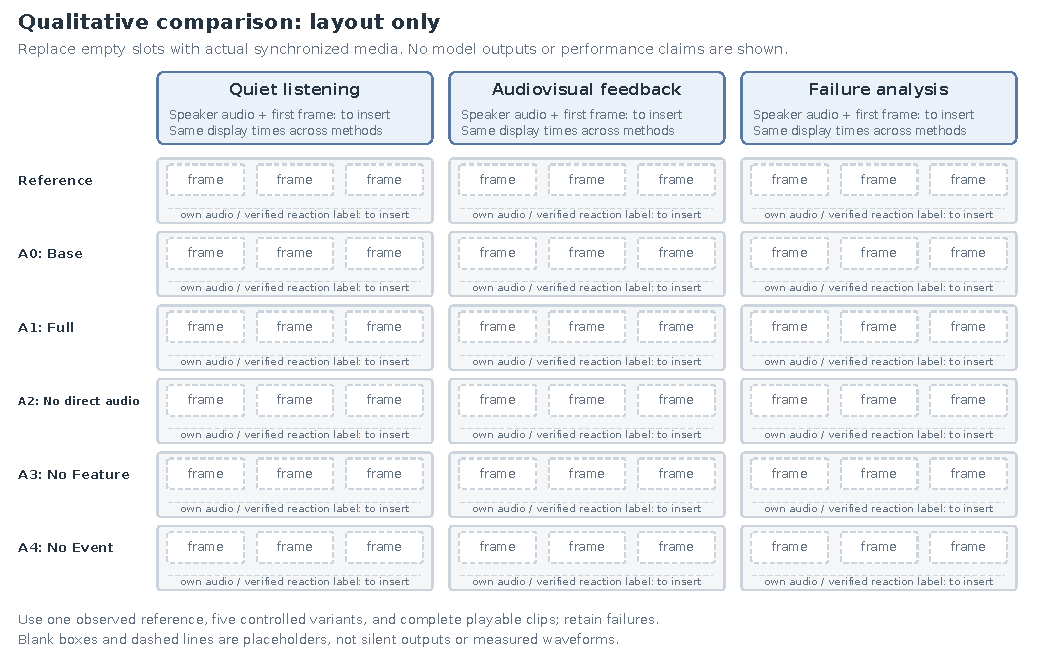
\includegraphics[width=\textwidth]{F5_results_layout.pdf}
\caption{\figdraft{F5: Qualitative comparison layout only} Three planned cases cover quiet listening, audiovisual feedback, and failure analysis. Rows reserve space for a reference response and the five ablation configurations. Every frame and audio slot is empty: this figure contains no generated result or claimed performance difference.}
\label{fig:qualitative}
\end{figure*}

\paragraph{Human evaluation.}
\cnnote{人工评价计划}{在相同当前speaker音频与listener首帧条件下，匿名随机排序并由多位评分者判断适当性、参与感／自然度与声画协调（\cref{tab:human}）。画面／声音技术质量可分开评分。参考回应不是唯一正确答案，合理安静允许存在；无发声样本的相关协调项按协议记N/A并报告覆盖。人工仍需检查反应抢先、拖长或内部矛盾，不要求复现唯一GT时刻。}
\cnnote{统计计划}{使用配对设计，按来源对话处理片段相关性，报告置信区间与有效样本。单次生成seed如实注明；样本bootstrap不替代训练多seed的不确定性。评分人数、量表／A-B形式及一致性统计待确定，不能预设自动指标与人评高度相关。}
\begin{table*}[t]
\centering\small
\caption{T4: Human-evaluation layout. Dimensions are agreed; the rating scale, sampling, and uncertainty estimator are not finalized. Video-only methods are assessed only on applicable dimensions. No human scores have been filled.}
\label{tab:human}
\begin{tabularx}{\textwidth}{@{}Yccccc@{}}
\toprule
Method / comparison & \makecell{Contextual\\appropriateness} & \makecell{Engagement /\\naturalness} & \makecell{Audiovisual\\coordination} & \makecell{Valid\\samples} & Uncertainty \\
\midrule
A0: Base & \pending & \pending & \pending & \pending & \pending \\
A1: Full & \pending & \pending & \pending & \pending & \pending \\
Qwen$\rightarrow$OVI & \pending & \pending & \pending & \pending & \pending \\
GLARE & \pending & \pending & \NA & \pending & \pending \\
DyStream & \pending & \pending & \NA & \pending & \pending \\
Avatar Forcing & \pending & \pending & \NA & \pending & \pending \\
\bottomrule
\end{tabularx}
\cnnote{人工协议待确定}{正式名单随基线完成情况调整。需要补每条评分人数、评分者总数、一致性与置信区间。若使用A/B偏好则保留平局，若使用等级量表则补评分锚点。视觉方法与AV方法只在共同适用维度和明确展示条件下比较；安静样本不能自动获得声画协调满分。}
\end{table*}


\subsection{Ablation Studies}
\label{sec:ablation}
% Paragraph role P07: 五组消融定义
\Cref{tab:ablation} defines five configurations: a base model, the full model, and three variants that each remove one component. W denotes the additional Whisper cross-attention path, F denotes the two feature-supervision objectives, and E denotes clip-level event supervision on LTX hidden states. All configurations retain Qwen/Gemma conditions and the AV objective. Thus, the base model still receives speaker information and is not an unadapted LTX model.

% Paragraph role P08: 组件问题及五组结论边界
The W comparison asks whether direct acoustic information helps beyond the original Qwen conditions. The F comparison concerns the quality of generated media under target-feature supervision. The E comparison concerns omitted feedback categories and inappropriate extra activations. These are questions for evaluation, not established gains. Five configurations assess each component's conditional contribution within the full system and the overall change from the base; they do not isolate all component interactions or establish additive gains.
\begin{table*}[t]
\centering\small
\caption{T3: Five confirmed ablation configurations (result layout). W is the additional Whisper cross-attention path; F is the pair of feature objectives; E is clip-level event supervision on LTX hidden states. Every row retains Qwen/Gemma conditioning and AV training. Empty results do not imply an improvement.}
\label{tab:ablation}
\begin{tabularx}{\textwidth}{@{}Ycccrrrrrr@{}}
\toprule
Configuration & W & F & E & FID$\downarrow$ & FVD$\downarrow$ & \makecell{Visual\\mF1$\uparrow$} & \makecell{Audio\\mF1$\uparrow$} & \makecell{Miss$\downarrow$\\(\%)} & \makecell{False$\downarrow$\\(\%)} \\
\midrule
A0: Base & \off & \off & \off & \pending & \pending & \pending & \pending & \pending & \pending \\
A1: Full & \on & \on & \on & \pending & \pending & \pending & \pending & \pending & \pending \\
A2: Without direct audio & \off & \on & \on & \pending & \pending & \pending & \pending & \pending & \pending \\
A3: Without Feature & \on & \off & \on & \pending & \pending & \pending & \pending & \pending & \pending \\
A4: Without Event & \on & \on & \off & \pending & \pending & \pending & \pending & \pending & \pending \\
\bottomrule
\end{tabularx}
\cnnote{正式填写要求}{表中只固定五组结构，分数留空。P/R、逐类支持、适用音质与人评见配套细表，不以单个F1概括全部效果。各组固定规划器、训练数据、初始化、预算和采样；旧U-Event结果及SFT规划器变体不能直接填入。}
\end{table*}

\cnnote{受控条件与证据}{固定数据、标签、初始化、规划器、训练样本展示量和采样；可预生成同一预测描述供五组共用。训练仍用标注描述，测试用预测描述；GT描述对照另标oracle。W不能只用画质证明语义／韵律利用，F不能只用teacher重建损失证明最终媒体改善，E须同时看P/R/F1、误触发和合理安静倾听。}
\cnnote{历史结果与扩展}{旧U-Event的6000／8000和新LTX6000＋SFT2752结果均不能代替这五组正式同条件结果。监督位置、整段／时序、两路Feature拆分和权重网格暂列可选；只有新增相应独立主张时再安排对照。}


\subsection{Data and Evaluation Validation}
\label{sec:validation}
\paragraph{Data and annotation quality.}
\cnnote{资源与媒体抽检计划}{统计来源、角色、音轨、片段长度、人脸质量、有声／安静比例、逐类支持与共现。代表性随机抽检覆盖边界完整性、角色对应、音轨污染／过度截除和脸部可用性；稀有层过采样需按真实分布加权。资源分支关系放附录，正文保持最终规模简洁。}
\cnnote{配对标注核验计划}{固定同批片段、Qwen3-Omni版本、采样设置与输出要求，比较仅音视频与加入带时间线索的匿名描述（\cref{tab:annotation}）。独立人工核验遗漏、无依据添加、顺序与发声内容；同时报告正确性和完整性。已有24条有声试点只能说明观察来源。若要声称数据处理提升生成效果，另需固定模型、规模和预算的训练对照。}
\begin{table*}[t]
\centering\small
\caption{辅助标注质量表草案（待实施，可移至附录）。固定相同片段，对匿名描述进行独立人工核验；所有数值待填。}
\label{tab:annotation}
\begin{tabularx}{\textwidth}{@{}Yrrrrr@{}}
\toprule
标注设置 & 样本数 & 事件遗漏$\downarrow$ & 无依据添加$\downarrow$ & 顺序错误$\downarrow$ & 发声描述错误$\downarrow$ \\
\midrule
仅音视频 & \pending & \pending & \pending & \pending & \pending \\
音视频＋带时间反应线索 & \pending & \pending & \pending & \pending & \pending \\
\bottomrule
\end{tabularx}
\cnnote{统计口径待补}{各项分母、判定标准和分层抽样方式需先定义。检测线索不是人工真值；更长描述不直接表示更准确。媒体质量抽检另记录角色／切分合格率、音轨问题和脸部可用性。}
\end{table*}


\paragraph{Event-evaluator reliability.}
\cnnote{事件评测器核验}{在真实和生成媒体上分别抽样核验外部检测器，覆盖有声／无声、常见／稀有类及失败例；报告逐类质量、支持数和覆盖。训练弱负例不直接当测试负真值，未知／失败不当正确安静；不能用训练Event头自评。}
\cnnote{本小节作用}{这里核验数据与测量工具是否可信；生成效果由主对比和消融回答，用户感受由前述人工评价回答。完成核验后报告具体发现，详细错误清单和逐类结果可放补充材料。}
\cnnote{可选扩展与范围}{Whisper置零／错配、GT描述oracle、多seed、时长／发声／脸部质量分层和完整推理开销仅为可选诊断。错配可能产生条件冲突，不能单独证明理解；多样性需同时看适当性，不选best-of-N。推理开销包括描述、重编码、各编码器、生成与解码，不将片段吞吐叫流式延迟。本阶段不增加多轮历史、persona保持、全身或实时流式主张。}
\cnnote{已有证据状态，按中文稿快照}{ViCo43已完成历史联合8000、DyStream和Avatar Forcing自动比较，人工评分为0；双200 LTX6000＋SFT2752有视频与活动结果，UTMOSv2无有效窗口，SyncNet／GLARE未运行；基础AV训练已启动，不能称五组完成。上述记录仅作筹备依据，当前不填正式结果表。}

\section{Conclusion}
\label{sec:conclusion}
\cnnote{结论待写}{正式结果尚未汇齐。完成主对比、五组消融、数据质量及评价核验后，再根据实际证据写结论；当前不新增性能、泛化或交互体验提升的结论。}
\paragraph{Limitations and future work.}
\cnnote{局限段落待写}{结果确定后，用一个短段落结合失败例说明适用边界。当前设定只使用当前语音与首帧；自动标注、外部事件检测及单一参考评价的局限需结合核验结果说明。这里不新增多轮历史、人物长期一致性或实时流式实验要求。}
\cnnote{作者自查}{贡献：保留数据、模型和评价三条方向，效果证据待补。写作：已区分标注／生成模型、训练／推理描述和两类事件协议。实验：五组已规划，成绩留空。评价：外部检测、人工规范和覆盖待落实。方法：冻结基座及梯度路径已说明，版本与细节待核对。完整逐项核对见review/含义与证据核对.md。}

\clearpage
\cnnote{引用占位}{以下参考文献仅用已知工作名称标识引用对象，不是正式书目信息。请按 CITATIONS.md 下载原始 BibTeX，替换 references.bib 中同名键；不依据文件名补作者、年份或录用会议。}
{\small\bibliographystyle{ieeenat_fullname}\bibliography{references}}
\end{document}
